\documentclass{article}
\usepackage{graphicx}
\usepackage[margin=1in]{geometry}
\usepackage[outdir=./]{epstopdf}  					% Avoids errors when input figures
\usepackage[labelsep=period,labelfont=bf]{caption}
%\usepackage{subcaption}

\begin{document}
\begin{figure}[tbph]
\caption{Connectedness of Emerging Market 10-Year Yields} \label{fig:dyindex10y}
\begin{center}
	\begin{minipage}{0.9\linewidth}
	\begin{center}
	\begin{subfigure}[t]{\linewidth}
			\includegraphics[trim={0cm 0cm 0cm 0cm},clip,height=0.34\textheight,width=\linewidth]{../Figures/Estimation/dy_index_dn_data.eps} \\
			\vspace{-0.35cm}
			\caption{Nominal and Synthetic Yields} \label{subfig:dyindex10ynomsyn}
			\vspace{0.4cm}
	\end{subfigure}
	
	\begin{subfigure}[t]{\linewidth}
			\includegraphics[trim={0cm 0cm 0cm 0cm},clip,height=0.34\textheight,width=\linewidth]{../Figures/Estimation/dy_index10y_dcmp.eps} \\
			\vspace{-0.35cm}
			\caption{Nominal Yield Components} \label{subfig:dyindex10ydcmp}
	\end{subfigure}
	\end{center}
	\fignotes{This figure plots the connectedness index of \cite{DieboldYilmaz:2014} for the 10-year nominal yields of emerging markets. Panel (a) compares the connectedness of nominal yields (solid line) against that of synthetic yields (dashed-dotted line) and the nominal yields of advanced countries (dashed line). Panel (b) compares the connectedness of each component of the nominal yields: the expected future short rate (solid line), the term premium (dashed-dotted line) and the credit risk compensation (dashed line). The index is obtained using a vector autoregression of order 1, with a forecast horizon of 10 days and a rolling window of 150 days for the daily changes of the 10-year nominal yields and each of their components. The index for some components has a shorter history because its computation requires a balanced panel and the components do not start on the same date (e.g. the construction of the synthetic curves does not involve nominal yields).}
	\end{minipage}
\end{center}
\end{figure}
\end{document}
% trim = {<left> <lower> <right> <upper>}